\begin{figure}[H]
	\centering
	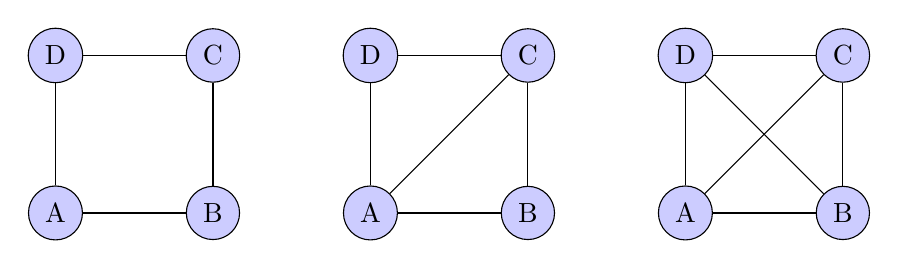
\begin{tikzpicture}
		% Quadrato - Clustering coefficient = 0
		\node[circle, draw, fill=blue!20] (A1) at (0,0) {A};
		\node[circle, draw, fill=blue!20] (B1) at (2,0) {B};
		\node[circle, draw, fill=blue!20] (C1) at (2,2) {C};
		\node[circle, draw, fill=blue!20] (D1) at (0,2) {D};
		\draw (A1) -- (B1);
		\draw (B1) -- (C1);
		\draw (C1) -- (D1);
		\draw (D1) -- (A1);
		
		% Quadrato con diagonale - Clustering coefficient = 5/6
		\node[circle, draw, fill=blue!20] (A2) at (4,0) {A};
		\node[circle, draw, fill=blue!20] (B2) at (6,0) {B};
		\node[circle, draw, fill=blue!20] (C2) at (6,2) {C};
		\node[circle, draw, fill=blue!20] (D2) at (4,2) {D};
		\draw (A2) -- (B2);
		\draw (B2) -- (C2);
		\draw (C2) -- (D2);
		\draw (D2) -- (A2);
		\draw (A2) -- (C2); % Diagonale
		
		% Grafo completo - Clustering coefficient = 1
		\node[circle, draw, fill=blue!20] (A3) at (8,0) {A};
		\node[circle, draw, fill=blue!20] (B3) at (10,0) {B};
		\node[circle, draw, fill=blue!20] (C3) at (10,2) {C};
		\node[circle, draw, fill=blue!20] (D3) at (8,2) {D};
		\draw (A3) -- (B3);
		\draw (A3) -- (C3);
		\draw (A3) -- (D3);
		\draw (B3) -- (C3);
		\draw (B3) -- (D3);
		\draw (C3) -- (D3);
	\end{tikzpicture}
	\caption{Clustering coefficient examples: on the left a graph with clustering coefficient equal to zero; on the center, a graph with clustering coefficient equal to 5/6, on the right a graph with clustering coefficient equal to 1.}
	\label{fig:clustering-coefficient-examples}
\end{figure}
